% +------------------------------------+
% |   Generated by www.docx2latex.com  |
% |   Version: 2.0.0                   |
% +------------------------------------+

\documentclass[11pt]{book}

\usepackage{adjustbox}
\usepackage{caption}
\usepackage{float}
\usepackage[T1]{fontenc}
\usepackage{graphicx}
\usepackage{hhline}
\usepackage[utf8]{inputenc}
\usepackage{multicol}
\usepackage{multirow}
\usepackage{subcaption}
\usepackage[normalem]{ulem}
\usepackage[paperheight=29.69cm,paperwidth=21.01cm,left=2.54cm,right=2.54cm,top=2.54cm,bottom=2.54cm]{geometry}
\usepackage[hidelinks]{hyperref}


\setlength\parindent{0pt}
\renewcommand{\arraystretch}{1.3}


\title{9 New Hypothesis -Probabilistic Model of Spatial Alignment Success}

\begin{document}
\maketitle

In this chapter, we will explore the concept of ``\textbf{Successful Alignment}" as a sub-problem of "Successful Assembly" and model it with a probabilistic approach. After observing the construction of the three demonstration structures, assembly success is dependent on two main factors: good alignment and high assembly force. While assembly force is specific to the assembly of integral timber joints, alignment is a generic challenge that affects all assembly processes, particularly those involving spatial assembly.

A robotic assembly process can be seen as a continuous chain of automatic operations. Within this chain, there are certain critical moments where good alignment accuracy is crucial before the process can continue successfully. By seeing every one of these moments as a challenge, where there is a certain probability of success, we can understand the overall ``Successful Assembly" as a combination of discrete probabilistic events.

\textbf{Alignment accuracy}, being a prerequisite for successful assembly, was a core challenge throughout this thesis, appearing in various forms and addressed at multiple stages of development. The initial focus was on aligning timber joints with each other to ensure proper closure, leading to the development of chamfered joint edges and high-force robotic clamps for passive guidance. \textit{(see \uline{5.6.6 Clamping Joints with Chamfered Edges})} As the research progressed towards automatic DiRT tool placement, additional alignment scenarios were required to attach and detach tools automatically, presenting unique challenges and necessitating the development of active correction methods \textit{(see \uline{7.3.14 Camera-Marker Alignment Correction System})}.

Reflecting on the three demonstrator construction, it became apparent that alignment and corrections were not always successful, as deviations could be larger than expected. This prompted an investigation into the sources of these deviations and the potential for developing models to better predict them. Towards the end of this thesis, after examining all alignment scenarios, a pattern for modelling the alignment and correction problem emerged. This led to a new hypothesis—a statistical model capable of predicting the probability of successful alignment by considering deviation, tolerance, and the correction method applied.

In this chapter, I will introduce the new hypothesis centred around the probabilistic model of spatial alignment success and explore its implications for the broader assembly domain. It is important to note that this model has not been tested within the scope of this thesis but the current findings shows that the model is in agreement with the observations. Further studies are required to confirm its completeness, validity, and practicality. 

\subsection{Modelling Alignment and Correction}

Let's begin by looking at the following table that outlines all the alignment scenarios performed. Since we are using one robot for the assembly, the scenarios can all be described as ``Some part(s) on the robot-side attempting to align with some other part(s) on the stationary-side". 

\begin{table}[H]
\begin{adjustbox}{max width=\textwidth}
\begin{tabular}{p{1.22cm}p{5.13cm}p{3.94cm}p{3.89cm}p{1.72cm}}
\hline
\multicolumn{1}{|p{1.22cm}}{{\footnotesize \textbf{Type}}} & 
\multicolumn{1}{|p{5.13cm}}{{\footnotesize \textbf{Robot side}}} & 
\multicolumn{1}{|p{3.94cm}}{{\footnotesize \textbf{Stationary Side}}} & 
\multicolumn{1}{|p{3.89cm}}{{\footnotesize \textbf{Purpose of Alignment}}} & 
\multicolumn{1}{|p{1.72cm}|}{{\footnotesize \textbf{Since Dev’ Phase}}} \\ 
\hline
\multicolumn{1}{|p{1.22cm}}{{\footnotesize \textbf{1}}} & 
\multicolumn{1}{|p{5.13cm}}{{\footnotesize \textbf{Timber joint} on beam held by robot}} & 
\multicolumn{1}{|p{3.94cm}}{{\footnotesize \textbf{Timber joint} on the partially built timber structure}} & 
\multicolumn{1}{|p{3.89cm}}{{\footnotesize Before joint closure by clamp(s)}} & 
\multicolumn{1}{|p{1.72cm}|}{{\footnotesize 2}} \\ 
\hline
\multicolumn{1}{|p{1.22cm}}{{\footnotesize \textbf{2}}} & 
\multicolumn{1}{|p{5.13cm}}{{\footnotesize \textbf{Clamp }held by robot}} & 
\multicolumn{1}{|p{3.94cm}}{{\footnotesize \textbf{Clamp attachment holes} on the partially built timber structure}} & 
\multicolumn{1}{|p{3.89cm}}{{\footnotesize Before attaching clamp to partially build timber structure}} & 
\multicolumn{1}{|p{1.72cm}|}{{\footnotesize 3}} \\ 
\hline
\multicolumn{1}{|p{1.22cm}}{{\footnotesize \textbf{3}}} & 
\multicolumn{1}{|p{5.13cm}}{{\footnotesize \textbf{ATC (Robot Side) }on robot flange}} & 
\multicolumn{1}{|p{3.94cm}}{{\footnotesize \textbf{ATC (Tool Side) on Clamp} attached to already-build timber structure}} & 
\multicolumn{1}{|p{3.89cm}}{{\footnotesize Before docking with clamp to retrieve it after use}} & 
\multicolumn{1}{|p{1.72cm}|}{{\footnotesize 3}} \\ 
\hline
\multicolumn{1}{|p{1.22cm}}{{\footnotesize \textbf{4}}} & 
\multicolumn{1}{|p{5.13cm}}{{\footnotesize \textbf{Clamp }held by robot}} & 
\multicolumn{1}{|p{3.94cm}}{{\footnotesize \textbf{Tool Storage Rack }at fixed location}} & 
\multicolumn{1}{|p{3.89cm}}{{\footnotesize Before returning clamp to storage rack}} & 
\multicolumn{1}{|p{1.72cm}|}{{\footnotesize 3}} \\ 
\hline
\multicolumn{1}{|p{1.22cm}}{{\footnotesize \textbf{5}}} & 
\multicolumn{1}{|p{5.13cm}}{{\footnotesize \textbf{ATC (Robot Side) }on robot flange}} & 
\multicolumn{1}{|p{3.94cm}}{{\footnotesize \textbf{ATC (Tool Side) on Clamp on Tool Storage Rack }at fixed location} \newline
} & 
\multicolumn{1}{|p{3.89cm}}{{\footnotesize Before retrieving clamp from storage rack}} & 
\multicolumn{1}{|p{1.72cm}|}{{\footnotesize 3}} \\ 
\hline
\multicolumn{1}{|p{1.22cm}}{{\footnotesize \textbf{6A}}} & 
\multicolumn{1}{|p{5.13cm}}{{\footnotesize \textbf{Screw Tip on Screwdriver }held by robot}} & 
\multicolumn{1}{|p{3.94cm}}{\multirow{2}{*}{\parbox{3.94cm}{{\footnotesize \textbf{Pre-drilled Screw Hole} on beam with the rest of partially built timber structure} \newline
}}} & 
\multicolumn{1}{|p{3.89cm}}{\multirow{2}{*}{\parbox{3.89cm}{{\footnotesize Before joint closure by screwdriver(s)}}}} & 
\multicolumn{1}{|p{1.72cm}|}{\multirow{2}{*}{\parbox{1.72cm}{{\footnotesize 4}}}} \\ 
\hhline{--~~~}
\multicolumn{1}{|p{1.22cm}}{{\footnotesize \textbf{6B}}} & 
\multicolumn{1}{|p{5.13cm}}{{\footnotesize \textbf{Screw Tip on Screwdriver attached to flying beam }held by robot}} & 
\multicolumn{1}{|p{3.94cm}}{} & 
\multicolumn{1}{|p{3.89cm}}{} & 
\multicolumn{1}{|p{1.72cm}|}{} \\ 
\hline
\multicolumn{1}{|p{1.22cm}}{{\footnotesize \textbf{7}}} & 
\multicolumn{1}{|p{5.13cm}}{{\footnotesize \textbf{ATC (Robot Side) }on robot flange}} & 
\multicolumn{1}{|p{3.94cm}}{{\footnotesize \textbf{ATC (Tool Side) on Screwdriver }attached to already-build timber structure}} & 
\multicolumn{1}{|p{3.89cm}}{{\footnotesize Before docking with screwdriver to retrieve it after use}} & 
\multicolumn{1}{|p{1.72cm}|}{{\footnotesize 4}} \\ 
\hline
\multicolumn{1}{|p{1.22cm}}{{\footnotesize \textbf{8}}} & 
\multicolumn{1}{|p{5.13cm}}{{\footnotesize \textbf{Screwdriver }held by robot}} & 
\multicolumn{1}{|p{3.94cm}}{{\footnotesize \textbf{Tool Storage Rack }at fixed location}} & 
\multicolumn{1}{|p{3.89cm}}{{\footnotesize Before returning the screwdriver to the storage rack. \\ $\ast$}} & 
\multicolumn{1}{|p{1.72cm}|}{{\footnotesize 4}} \\ 
\hline
\end{tabular}
\end{adjustbox}
\end{table}
\vspace{6\baselineskip}
{\footnotesize $\ast$ Note that the attachment of the screwdriver to the new beam is performed manually by the operator, no robotic alignment is performed.\par}

{\footnotesize $\ast$ Type $\#$6A and $\#$6B both occur at the same moment during the alignment of the screwdrivers. $\#$6A refers to the screwdriver that is held directly by the robot, while $\#$6B refers to the other screwdrivers that are hanging from the flying beam. (see \uline{7.5.2.2 Screwdriver as a Gripper})\par}

\subsubsection{Alignment-Correction Model}

Observations of the three demonstrations (from Development Phase 3 to 5) indicated that there are many different factors affecting the amount of deviation in each of the alignment scenarios. They affect whether the total pairwise deviation can be corrected and thus the chance of successful assembly. Below are some examples of the success factors:

\begin{itemize}
	\item \textbf{Tight tolerance, deviation of partially assembled structure :} When picking up tools from the structure (types $\#$3 and $\#$7), the alignment between robot-side ATC and tool-side ATC has a very low chance of success\textit{ (see \uline{6.5.3 Docking Adapter Misalignment})}. This may be caused by a combination of the small allowable tolerance (2mm) governed by the design of the ATC and the high deformation of the partially built structure from which the tool is hanging. 

	\item \textbf{Correction range: }Comparing the two joint closure methods, screwing closure (type $\#$6) have a much higher success rate than clamping closure (type $\#$1). This may be explained by the pointy tip of the screwdriver aiming at a relatively large pre-drilled hole.

	\item \textbf{Deviation:} When retrieving tools from and returning tools to the stationary tool storage (type $\#$4, $\#$5 and $\#$8), the alignment has a very high success rate when compared to other alignment types. This may be explained by the fact that tool storage alignment is performed manually by teaching, there is no deviation of the tool storage afterwards and the robotic platform is repeatable. In other alignment scenarios, the target is novel and may be deformed from its designated location.

	\item \textbf{Payload: }During the transport of a beam to the work area, if the beam is very heavy \textit{(see \uline{7.5.5 Heavy Beam Caused Robot Overload})}, or if the grasp is not near the middle, the chance of success is low. 

\end{itemize}
In order to create a unified model to include different deviation factors, I first draw inspiration from the study of error in machine design, which uses the concept of structural loop to identify sources of error.

\begin{figure}[H]
\includegraphics[width=15.92cm,height=9.98cm]{./images/image1.jpeg}
\end{figure}


The diagram above shows a Type 1 alignment scenario where two joints needs to be aligned. We can identify two \textbf{structural chain }that stems from a fixed reference (ground or ceiling) towards the two points of alignment \href{https://www.zotero.org/google-docs/?vXepVQ}{(Slocum, 1992)}. On the robot-side, the timber joint is located on a beam held by the robot through a gripper. On the stationary-side, the timber joint is located on the partially built timber structure, which is located on a temporary platform. In a perfect scenario, the alignment point (or pose) on each side should both be equal to the target that is extracted from the CAD model. I refer to this as the ‘\textbf{ground truth}’. In reality, due to imperfection of each component in the structural loop, both alignment points will be deviated from the ground truth. These imperfections include stiffness of the timber material, accuracy of the prefabricated timber parts, deformation of the machine parts and inaccuracy of the robotic control systems. 

The second inspiration is taken from the study of reliability in the field of systems engineering, for the use of probability to model success and failure \href{https://www.zotero.org/google-docs/?zmsGMJ}{(Hallmann et al., 2020)}.\textit{ }Consider the deviation between the two alignment points, we can assume it behaves like a random variable. This allows us to model it as a continuous probability distribution that can be analysed using statistical methods. Specifically, using the cumulative distribution function\footnote{ In probability theory and statistics, the cumulative distribution function (CDF) of a real-valued random variable X, evaluated at x, is the probability that X will take a value less than or equal to x. } (CDF) to analyse the worst-case deviation.

The two graphs below can help us understand CDF in a graphical way. Let us consider the deviations between the two alignment points. Assuming it is a continuous random variable, its distribution can be graphed using the probability density function, where the X axis is the deviation and Y axis is the probability density. The area under the graph represents all possible values, and therefore it has an area of 1. If we want to find the probability that the actual deviation is less than a certain threshold, we can draw a vertical line at that threshold and find the area on the left-hand side. Mathematically, this can be represented by \textbf{F\textsubscript{D}(x) $=$ P (D$\leq$x)}, where \textbf{F\textsubscript{D}() is the CDF of deviation D}, P is the probability density function (PDF), and the T is the threshold to be analysed.

In practice, it is possible to quantify the PDF of a random variable by measurement, model fitting and simulation. Details of which will be presented later in the section.

\begin{figure}[H]
\includegraphics[width=15.92cm,height=7.94cm]{./images/image2.jpeg}
\end{figure}


\vspace{1\baselineskip}
The use of PDF and CDF is related to, but different from the typical accuracy representation in the field of robotics. When discussing machine accuracy, it is more common to measure trueness (difference between ground truth and statistical mean) and precision (standard deviation of the distribution). 

However, for the purpose of assembly, we are interested in the \textbf{worst-case deviation }between the two alignment points for determining whether the alignment is sufficiently good. The use of CDF allows us to directly model the alignment problem by relating the threshold value and the probability of the actual value falling within range. 

Given the following variables: 

\begin{itemize}
	\item \textbf{d }is the measured deviation of the two alignment points across the open structural loop. It is assumed to be a random variable because of the random imperfections in the system. 

	\item \textbf{D} is the probability distribution of the random deviation d, 

	\item \textbf{x} is a variable representing a deviation threshold to be analysed 

	\item \textbf{K\textsubscript{D }$\in$ (0, 1) }represents the probability that the \textbf{d} takes on a value less than or equal to \textbf{x}. 

\end{itemize}
Using the cumulative distribution function \textbf{F\textsubscript{D}(),} we can define a variable \textbf{K\textsubscript{D }$\in$ (0, 1) }to be the probability that the \textbf{d} takes on a value less than or equal to \textbf{x}: 

\textbf{K\textsubscript{D} $=$ F\textsubscript{D}(x) $\ldots$$\ldots$$\ldots$$\ldots$$\ldots$$\ldots$$\ldots$$\ldots$$\ldots$$\ldots$$\ldots$$\ldots$$\ldots$$\ldots$$\ldots$$\ldots$$\ldots$. [1]}

In addition, we model the \textbf{allowable assembly tolerance} of the mating features, such as the gap in a pin-in-hole assembly or the gap on a loose joint pair. From the perspective of the mating features, it is the maximum threshold of deviation d such that assembly is still successful. We can define it using: 

\begin{itemize}
	\item \textbf{T }as the allowable assembly tolerance 

\end{itemize}
If a \textbf{correction mechanism} is used, such as chamfered edges passive correction or camera-marker active correction. We can model the properties of the correction mechanism or process using: 

\begin{itemize}
	\item \textbf{C\textsubscript{Range}} as the maximum correctable range (e.g. size of chamfered joint edge)

	\item \textbf{K\textsubscript{C}} \textbf{$\in$ (0, 1) }as the success rate of the correction method. 

\end{itemize}
\textbf{The numerical representation and units }have to be consistent for \textbf{d, x\textsubscript{ }}, \textbf{T, C\textsubscript{Range}} and \textbf{C\textsubscript{Residual}}. For the sake of simple arithmetics, the subsequent explanation will only consider the absolute Cartesian distance for the deviation. Therefore it is represented as a signless real number. Alternatively, a transformation consisting of translation and rotation can be used. However, the transformation arithmetics will be outside the scope of this explanation. 

Finally, the probability of successful assembly is represented by \textbf{S $\in$ (0, 1)}. Using the defined variables, I propose the following Alignment-Correction Model to relate S as a function of d with three intervals: 

\begin{enumerate}
	\item \textbf{No correction needed: if d $\leq$ T then S $=$ 1 \\ }(Explanation: No correction is needed because the deviation is within the allowable tolerance.)

	\item \textbf{Correction success: if T < d $\leq$ C\textsubscript{Range}} \\ (Explanation: The deviation is within the range of the correction mechanism and its residual deviation is within the allowable tolerance.)

	\item \textbf{Correction failure:} \textbf{if C\textsubscript{Range} < d then S $=$ 0}

\end{enumerate}
The function can be expressed by: 

\begin{table}[H]
\begin{adjustbox}{max width=\textwidth}
\begin{tabular}{p{1.64cm}p{0.74cm}p{1.27cm}p{3.55cm}p{1.53cm}}
\hhline{~~~~~}
\multicolumn{1}{p{1.64cm}}{\multirow{3}{*}{\parbox{1.64cm}{\centering
\textbf{S (d) $=$ }}}} & 
\multicolumn{1}{p{0.74cm}}{\multirow{3}{*}{\parbox{0.74cm}{\centering
{\fontsize{46pt}{55.2pt}\selectfont $\{$}}}} & 
\multicolumn{1}{p{1.27cm}}{\textbf{1}} & 
\multicolumn{1}{p{3.55cm}}{\textbf{if d $\leq$ T}} & 
\multicolumn{1}{p{1.53cm}}{\textbf{(I)}} \\ 
\hhline{~~~~~}
\multicolumn{1}{p{1.64cm}}{} & 
\multicolumn{1}{p{0.74cm}}{} & 
\multicolumn{1}{p{1.27cm}}{\textbf{K\textsubscript{C}}} & 
\multicolumn{1}{p{3.55cm}}{\textbf{if T < d $\leq$ C\textsubscript{Range }}} & 
\multicolumn{1}{p{1.53cm}}{\textbf{(II)}} \\ 
\hhline{~~~~~}
\multicolumn{1}{p{1.64cm}}{} & 
\multicolumn{1}{p{0.74cm}}{} & 
\multicolumn{1}{p{1.27cm}}{\textbf{0}} & 
\multicolumn{1}{p{3.55cm}}{\textbf{if C\textsubscript{Range} < d\textsubscript{ }}} & 
\multicolumn{1}{p{1.53cm}}{\textbf{(III)}} \\ 
\hhline{~~~~~}
\end{tabular}
\end{adjustbox}
\end{table}
\vspace{4\baselineskip}
\section{…………………………. ………………………… [2]}

Note that some correction mechanisms do not correct the deviation to zero but to within a certain range. It is important for this residual deviation after correction to be smaller than \textbf{T}, such that it can be accommodated by the allowable tolerance. In practice, the allowable tolerance and residual deviation are physical properties of the mating feature and the correction system, which can always be satisfied by proper design of the correction mechanism. For example, in the camera-marker correction system, the convergence value is designed to ensure successful alignment with the docking adapter.

Using the CDF of D, equation [1] , the probability of \textbf{d} landing inside interval I is 

\textbf{k\textsubscript{I} $=$ F\textsubscript{D}(T) $\ldots$$\ldots$$\ldots$$\ldots$$\ldots$$\ldots$$\ldots$$\ldots$$\ldots$$\ldots$. [3]}

For landing in interval II, 

\textbf{k\textsubscript{II} $=$ F\textsubscript{D}(C\textsubscript{Range}) - F\textsubscript{D}(T) $\ldots$$\ldots$$\ldots$$\ldots$$\ldots$$\ldots$$\ldots$$\ldots$$\ldots$$\ldots$. [4]}

The following diagram graphically represents the distribution of alignment points around the ground truth graphically. The two circles define the boundary between interval I and II and III. The radius of the inner circle is equal to the upper bound of interval I where d $=$ T, the radius of the outer circle is the upper bound of interval II where d $=$ C\textsubscript{Range}. . 

The graph on the right depicts the same concept, but plots the probability of successful assembly S(d) with respect to d and the labels are the probability of their occurrence from equations [3] and [4].

\begin{figure}[H]
\centering
\begin{subfigure}[b]{0.45\textwidth}
\centering
\includegraphics[width=\textwidth]{./images/image3.jpeg}
\end{subfigure}
\hfill
\begin{subfigure}[b]{0.45\textwidth}
\centering
\includegraphics[width=\textwidth]{./images/image4.jpeg}
\end{subfigure}
\end{figure}


We can find the combined probability of success \textbf{S }for all three zones. Note that interval III can be ignored because the probability of success is zero\textsubscript{. }

\textbf{S $=$ K\textsubscript{I} ⋅ S\textsubscript{I} + K\textsubscript{II} ⋅ S\textsubscript{II}}

\subsection{= FD(T) ⋅ 1 + (FD(CRange) - FD(T)) ⋅ Kc}

After arranging some terms:

\textbf{S $=$ F\textsubscript{D}(T) + F\textsubscript{D}(C\textsubscript{Range}) ⋅ K\textsubscript{c} - F\textsubscript{D}(T) ⋅ K\textsubscript{c}}

\textbf{S $=$ F\textsubscript{D}(T) (1 - K\textsubscript{c}) + F\textsubscript{D}(C\textsubscript{Range}) ⋅ K\textsubscript{c \ \ \ \ \ \ \ \ }$\ldots$$\ldots$$\ldots$$\ldots$$\ldots$$\ldots$$\ldots$$\ldots$$\ldots$$\ldots$$\ldots$$\ldots$$\ldots$$\ldots$ [5]}

In this thesis, in the cases where tight fitting joints are aligned with each other, there is zero tolerance (T $=$ 0) , thus \textbf{F\textsubscript{D}(T) $=$ 0.} In this special case, the formula can be simplified to:

\textbf{S $=$ F\textsubscript{D}(C\textsubscript{Range})⋅ K\textsubscript{C }\ \ \ \ \ \ \ \ $\ldots$$\ldots$$\ldots$$\ldots$$\ldots$$\ldots$$\ldots$$\ldots$$\ldots$$\ldots$$\ldots$$\ldots$$\ldots$$\ldots$ [6]}

\vspace{1\baselineskip}
\subsubsection{Application}

There are many ways that the model can be used. For example, to design a robotic system for a given structure with a \textbf{predictable success probability S}, it is possible to check all the alignment scenarios (after TAMP with the given robots and tools and design) within the process to determine its success probability. If we have N steps in a process, and each step has a success probability of S(N), and if success at each step is required for overall success, you can find the total probability of success by multiplying the success probabilities of each step together.

Total Probability of Success $=$ \textbf{S(1) ⋅ S(2) ⋅ ... ⋅ S(N) }

If we want to determine the average percentage of steps that are likely to succeed, we can do so by finding the average success probability across all steps. This can indicate how frequently an operator has to attend to an anomaly.

Average Success Probability $=$\textbf{ (S(1) + S(2) + ... + S(N)) / N }

Note that the distribution of D is dependent on the states of the robot and parts, and the value of T depends on the alignment scenario. Therefore the value of S is unique for each alignment in the entire process. It is easy for a computer to check all the alignment moments and visualise those with low success probability. This can help the production engineer identify problematic situations and take corrective actions. For example, to reduce the deformation of a partially-assembled structure by adding scaffolding, changing its assembly sequence or introducing diagonal bracing elements.

Another application is for designing the assembly details. We can identify if there is a systemically low success rate for a certain type of alignment. This may indicate that the tolerance or the correction mechanism for that type of scenario has to be adjusted. For example, by increasing the size of the edge chamfer or the field of view of the camera system. It is even possible to automatically assign the appropriate amount of edge chamfer to each joint until a satisfactory success rate is achieved.

It is also possible to use the model as a comparison tool when choosing robotic system components. For example, we can compare the implication of choosing a specific robotic arm, gantry, or docking adapter. 

In conclusion, the Alignment-Correction Model allows us to analyse and predict the success rate of various assembly alignment scenarios in a robotic process. By taking into account deviation, tolerance and the correction method, this model enables production engineers, system designers and structure designers to identify potential problems, make informed decisions and predict execution outcomes. It is generalisable, mathematically simple and can be implemented computationally to allow quick and comprehensive check of all the alignment scenarios. These factors are important to ensure an efficient fabrication-aware design process.

\subsubsection{Chaining Deviation}

In the previous section, we have assumed the deviation to be a probability distribution. In this section, we talk about the procedures to quantify this distribution. 

Refer to the structural loop diagram. We can see that each side of the open loop consist of a number of components between the fixed ground and the alignment point. Assuming each of these components are affected by random imperfections, each of them contribute to the deviation, and accumulate at the point of alignment. The total deformation on each link can therefore be modelled as a forward kinematics problem where the deviation caused by each component is modelled as a rigid transformation [Z] and the geometrical distance for each link is modelled as rigid transformation [X]. For a given chain P The general kinematic chain equation allows the deviation link to be computed:

\textbf{[T\textsubscript{P}] $=$ [Z\textsubscript{P1}][X\textsubscript{P1}][Z\textsubscript{P2}][X\textsubscript{P2}] $\ldots$ [X\textsubscript{Pn-1}][Z\textsubscript{Pn}] $\ldots$$\ldots$$\ldots$$\ldots$$\ldots$$\ldots$$\ldots$$\ldots$.. [7]}

Where total deviation between the two alignment points on chain P and Q can be found by:

d $=$ [T\textsubscript{P}][T\textsubscript{Q}]\textsuperscript{T}\textbf{ $\ldots$$\ldots$$\ldots$$\ldots$$\ldots$$\ldots$$\ldots$$\ldots$.. [8]}

While this representation of d using rigid transformation is quite accurate, the complex representation is hard to be used for statistical analysis. To simplify the analysis, we can consider only the absolute positional deviation in each of these components, which can be represented by a single number. In practice, the rotation component is often small enough and the Abby error associated with it is small. For a conservative analysis, the worst-case combined deviation of N links in the structural chain P can therefore be computed by:

d\textsubscript{P} $=$ d\textsubscript{P1} + d\textsubscript{P2} + $\ldots$ + d\textsubscript{PN} 

And the total deviation between the two alignment points on chain P and Q can be found by:

\textbf{d }$=$ d\textsubscript{P} + d\textsubscript{Q} \textbf{$=$ d\textsubscript{P1} + d\textsubscript{P2} + $\ldots$ + d\textsubscript{PN} + d\textsubscript{Q1} + d\textsubscript{Q2} + $\ldots$ + d\textsubscript{QN} }

Because of the simple summation, there is no more differentiation between the elements in either one of the chains. All the links can be treated in the same way. Therefore, for a structural loop with N links in total, d can be decomposed into:

\textbf{d $=$ d\textsubscript{1} + d\textsubscript{2} + $\ldots$ + d\textsubscript{N} \ \ \ \ \ \ \ \ $\ldots$$\ldots$$\ldots$$\ldots$$\ldots$. [9] }

Recall that each of the deviation components is a random statistical distribution, and they are independent of each other. We can expand the CDF of the total d into its constituting components. We can make use of the Joint Cumulative Distribution Function identity:

\textbf{F\textsubscript{XY}(x,y)$=$F\textsubscript{X}(x)F\textsubscript{Y}(y)}

For a structural loop with N links on both chains, the F\textsubscript{D}(d) evaluated at d can be expanded. 

\textbf{F\textsubscript{D}(d) $=$} \textbf{F\textsubscript{1}(d\textsubscript{1}) ⋅ F\textsubscript{2}(d\textsubscript{2}) ⋅ $\ldots$ ⋅ F\textsubscript{N}(d\textsubscript{N}) \ \ \ \ $\ldots$$\ldots$$\ldots$$\ldots$$\ldots$. [10] }

Where F\textsubscript{i}(d\textsubscript{i}) is the CDF of the link i evaluated at d\textsubscript{i}. Each of these distribution functions can be created from statistical measurements or by probabilistic simulation. Details of which will be presented later.

In conclusion, the simplification of the deviation from transformation to measuring only absolute distance, makes the computation of accumulated deviation much simpler. There are two major sources of inaccuracy. The first is an underestimation of error, because Abby error resulting from the chained rotational deviation is not considered. The second is an overestimation of error due to the summation of absolute distance compared to the transformation-based analysis using equations [7] and [8].

\begin{figure}[H]
\includegraphics[width=10.76cm,height=4.43cm]{./images/image5.jpeg}
\caption{can be used in equations [5] and [6] of the model. The relationship of d and d 1 , d 2 , $\ldots$, d N is described in equation [9]. During computation, an optimization function can be used to find the values of d 1 , d 2 , $\ldots$, d N such that it will maximise the result of the equation [13].}
\label{fig:can_be_used_equations_5}
\end{figure}


\vspace{1\baselineskip}
Depending on the nature of the deviation in the link, there are different methods of obtaining its statistical distribution. All of them require fitting a probability distribution to a series of measured data or properties. Different distributions can be selected depending on the shape of the measured data as long as an effective CDF can be applied to the distribution. Below are some examples of simple deviations and how they can found:

\begin{table}[H]
\begin{adjustbox}{max width=\textwidth}
\begin{tabular}{p{3.39cm}p{3.12cm}p{9.37cm}}
\hline
\multicolumn{1}{|p{3.39cm}}{{\scriptsize \textbf{Source of error}}} & 
\multicolumn{1}{|p{3.12cm}}{{\scriptsize \textbf{Dependent on Assembly State }}} & 
\multicolumn{1}{|p{9.37cm}|}{{\scriptsize \textbf{Measurement Technique}}} \\ 
\hline
\multicolumn{1}{|p{3.39cm}}{{\scriptsize Deviations in mechanical parts from designed form.  \\ (CAD to real error)}} & 
\multicolumn{1}{|p{3.12cm}}{{\scriptsize No}} & 
\multicolumn{1}{|p{9.37cm}|}{{\scriptsize Manufacturing tolerances are typically specified during production and can be treated as an absolute deviation. Alternatively, the manufactured part can be measured with measuring tools, the measured deviation is likely to be more accurate than those specified by the drawings. Remember to take into account the measuring tool’s accuracy. \par}} \\ 
\hline
\multicolumn{1}{|p{3.39cm}}{{\scriptsize Deviation of the timber parts due to cutting process}} & 
\multicolumn{1}{|p{3.12cm}}{{\scriptsize No}} & 
\multicolumn{1}{|p{9.37cm}|}{{\scriptsize The absolute deviation can be based on manufacturing tolerance standards. This results in a step function. The resulting CDF should be a step function. For more accurate distribution, measurement can be performed on manufactured samples. (see later section about Estimating Deviations - Accuracy of Timber Parts)\par}} \\ 
\hline
\multicolumn{1}{|p{3.39cm}}{{\scriptsize Docking accuracy between docking adapter}} & 
\multicolumn{1}{|p{3.12cm}}{{\scriptsize No}} & 
\multicolumn{1}{|p{9.37cm}|}{{\scriptsize The absolute deviation can be extracted from manufacturer specification.}} \\ 
\hline
\multicolumn{1}{|p{3.39cm}}{{\scriptsize Deformation of the partially built structure }} & 
\multicolumn{1}{|p{3.12cm}}{{\scriptsize State of the partial assembly, attached supports, and loads }} & 
\multicolumn{1}{|p{9.37cm}|}{{\scriptsize Probabilistic structural analysis, physical measurement needed to calibrate the model. (see later section about Estimating Deviations - Deformation of Partially Assembled Structure)\par}} \\ 
\hline
\multicolumn{1}{|p{3.39cm}}{{\scriptsize Deformation of the robotic platform }} & 
\multicolumn{1}{|p{3.12cm}}{{\scriptsize Configuration of the robot, state of attached loads}} & 
\multicolumn{1}{|p{9.37cm}|}{{\scriptsize Probabilistic robotic deviation analysis, physical measurement needed to calibrate the model. (see later section about Estimating Deviations - Accuracy of Robotic Platform)\par}} \\ 
\hline
\end{tabular}
\end{adjustbox}
\end{table}
\vspace{1\baselineskip}
{\footnotesize $\ast$ For measurements that rely on extracting the maximum deviation from tolerance standards, we can treat the resulting distribution as a step function, where the likelihood of deviation below that threshold is random. \par}

Consider the following example of a type $\#$1 joint-to-joint alignment scenario. For simplicity sake, this example requires only one joint alignment. The photo depicts the connectivity chain on the robot side P and stationary side Q at the alignment moment. The possible source of deviation and their quantification method for all parts and interfaces are listed in Table $\ldots$ and Table $\ldots$. The estimated deviation d and the probability F(d) in the experiment setup is listed for the purpose of an example, they are not derived from actual measurement.

\begin{figure}[H]
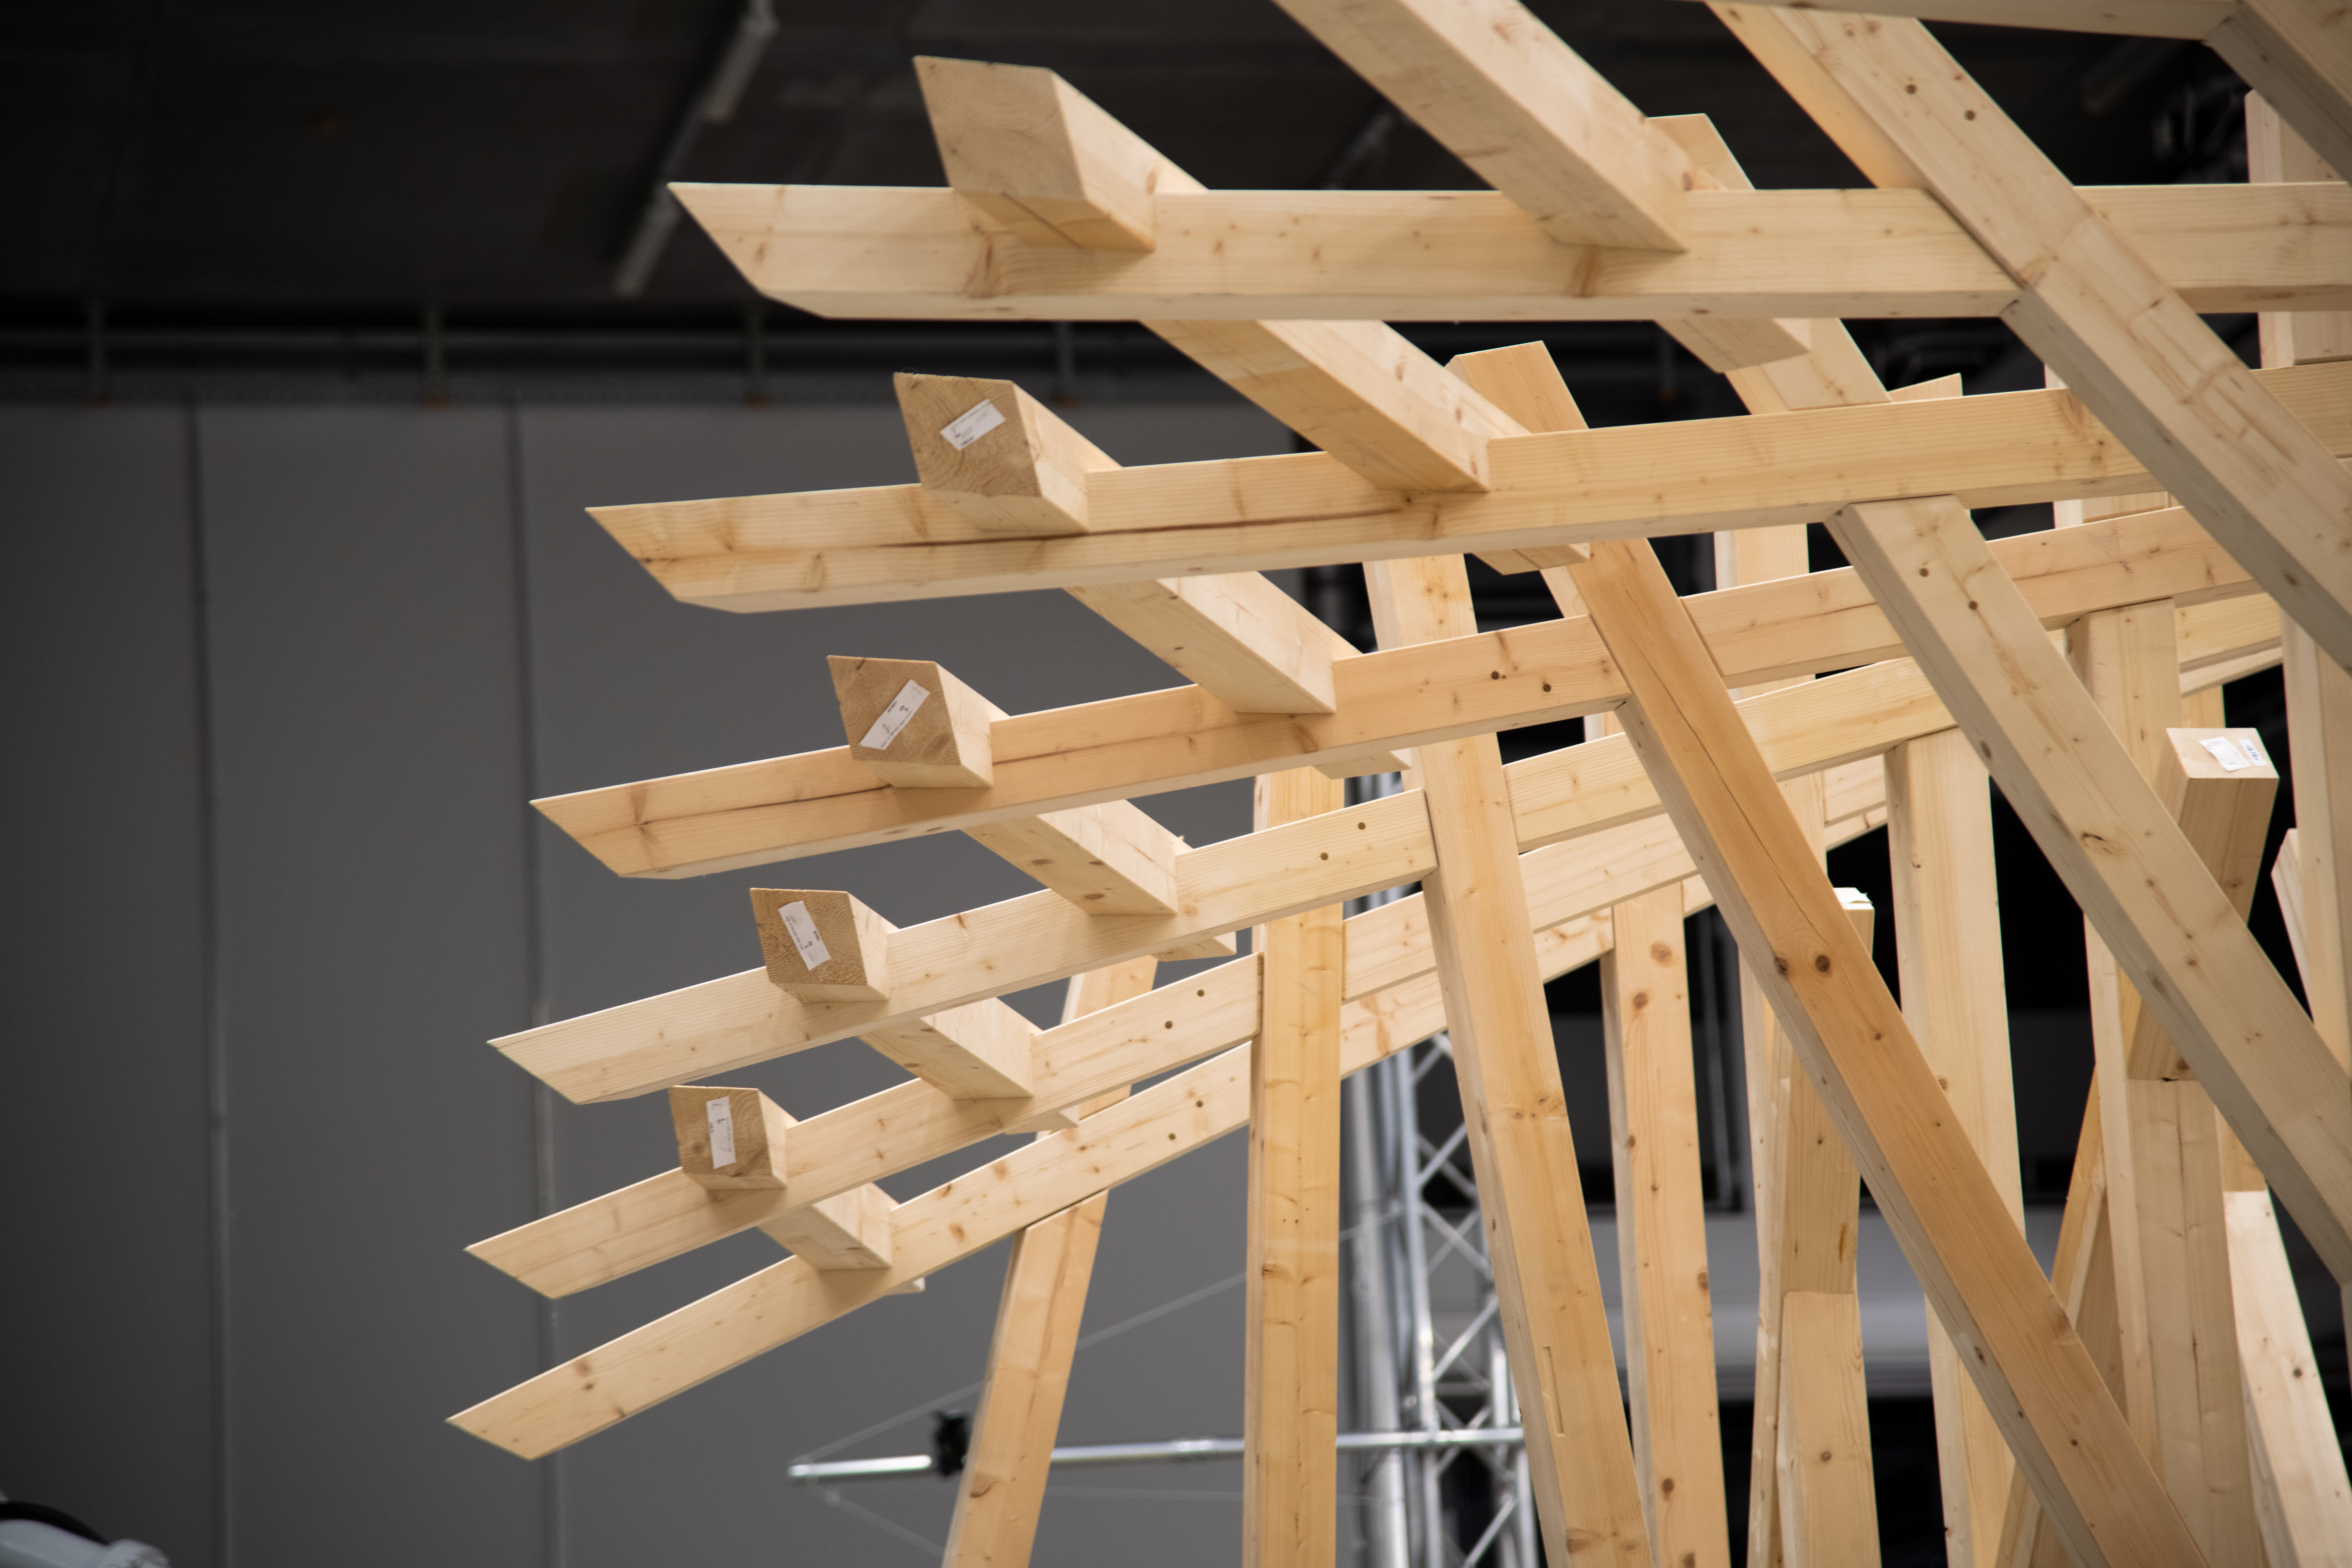
\includegraphics[width=15.92cm,height=8.96cm]{./images/image6.png}
\end{figure}


\begin{table}[H]
\begin{adjustbox}{max width=\textwidth}
\begin{tabular}{p{1.72cm}p{3.94cm}p{1.98cm}p{6.27cm}p{2.01cm}}
\hline
\multicolumn{1}{|p{1.72cm}}{{\scriptsize \textbf{Nature}}} & 
\multicolumn{1}{|p{3.94cm}}{{\scriptsize \textbf{Description }}} & 
\multicolumn{1}{|p{1.98cm}}{{\scriptsize \textbf{Deviation Fixed or State Dependent}}} & 
\multicolumn{1}{|p{6.27cm}}{{\scriptsize \textbf{Possible Source of Deviation and its Quantification Method}}} & 
\multicolumn{1}{|p{2.01cm}|}{{\scriptsize \textbf{Estimated d and F(d) in the experiment setup (mm)}}} \\ 
\hline
\multicolumn{1}{|p{1.72cm}}{{\scriptsize Interface}} & 
\multicolumn{1}{|p{3.94cm}}{{\scriptsize Robot to Ground Joint}} & 
\multicolumn{1}{|p{1.98cm}}{{\scriptsize Fixed}} & 
\multicolumn{1}{|p{6.27cm}}{{\scriptsize Difference between CAD Model and actual installation. Deviation can be measured by robot calibration procedure.\par}} & 
\multicolumn{1}{|p{2.01cm}|}{{\scriptsize 0.5 (1)}} \\ 
\hline
\multicolumn{1}{|p{1.72cm}}{{\scriptsize Part}} & 
\multicolumn{1}{|p{3.94cm}}{{\scriptsize Robot}} & 
\multicolumn{1}{|p{1.98cm}}{{\scriptsize State Dependent}} & 
\multicolumn{1}{|p{6.27cm}}{{\scriptsize Absolute accuracy of a robot with a fixed payload is often published by the manufacturer. } \newline
{\scriptsize Deformation of the robot body is dependent on pose and payload, it can be measured. \textit{(see Section - Accuracy of Robotic Platform for details)}\par}} & 
\multicolumn{1}{|p{2.01cm}|}{{\scriptsize 5 (0.95)}} \\ 
\hline
\multicolumn{1}{|p{1.72cm}}{{\scriptsize Interface}} & 
\multicolumn{1}{|p{3.94cm}}{{\scriptsize Robot Flange to ATC Joint}} & 
\multicolumn{1}{|p{1.98cm}}{{\scriptsize Fixed}} & 
\multicolumn{1}{|p{6.27cm}}{{\scriptsize Adapter plate manufacturing tolerance and installation inaccuracy. Deviation can be extracted from part production tolerance.\par}} & 
\multicolumn{1}{|p{2.01cm}|}{{\scriptsize 0.5 (1)}} \\ 
\hline
\multicolumn{1}{|p{1.72cm}}{{\scriptsize Part}} & 
\multicolumn{1}{|p{3.94cm}}{{\scriptsize ATC-R}} & 
\multicolumn{1}{|p{1.98cm}}{{\scriptsize Fixed}} & 
\multicolumn{1}{|p{6.27cm}}{\multirow{3}{*}{\parbox{6.27cm}{{\scriptsize ATC repeatability between robot and tool sides. (The combined repeatability between of the two ATC sides are often published by the manufacturer in their specification sheet)\par}}}} & 
\multicolumn{1}{|p{2.01cm}|}{\multirow{3}{*}{\parbox{2.01cm}{{\scriptsize 0.5 (1)}}}} \\ 
\hhline{---~~}
\multicolumn{1}{|p{1.72cm}}{{\scriptsize Interface}} & 
\multicolumn{1}{|p{3.94cm}}{{\scriptsize ATC Locking Interface}} & 
\multicolumn{1}{|p{1.98cm}}{{\scriptsize Fixed}} & 
\multicolumn{1}{|p{6.27cm}}{} & 
\multicolumn{1}{|p{2.01cm}|}{} \\ 
\hhline{---~~}
\multicolumn{1}{|p{1.72cm}}{{\scriptsize Part}} & 
\multicolumn{1}{|p{3.94cm}}{{\scriptsize ATC-T and Gripper}} & 
\multicolumn{1}{|p{1.98cm}}{{\scriptsize Fixed}} & 
\multicolumn{1}{|p{6.27cm}}{} & 
\multicolumn{1}{|p{2.01cm}|}{} \\ 
\hline
\multicolumn{1}{|p{1.72cm}}{{\scriptsize Interface}} & 
\multicolumn{1}{|p{3.94cm}}{{\scriptsize Gripper to Beam Interface}} & 
\multicolumn{1}{|p{1.98cm}}{{\scriptsize Fixed (with locating feature)} \newline
{\scriptsize State dependent (with friction gripper)}} & 
\multicolumn{1}{|p{6.27cm}}{{\scriptsize If a mechanical locating feature is used, the deviation is related to the design of the feature. For example the mechanical fit between a locating pin and the corresponding hole.\par} \newline
{\scriptsize If a friction-based gripper finger is used, the deviation is related to the amount and probability that the beam will slip inside the gripper. This may be dependent on beam weight, grasp orientation and grasp eccentricity.\par}} & 
\multicolumn{1}{|p{2.01cm}|}{{\scriptsize 0.5 (1)}} \\ 
\hline
\multicolumn{1}{|p{1.72cm}}{{\scriptsize Part}} & 
\multicolumn{1}{|p{3.94cm}}{{\scriptsize Lap Joint on Beam}} & 
\multicolumn{1}{|p{1.98cm}}{{\scriptsize State dependent }} & 
\multicolumn{1}{|p{6.27cm}}{{\scriptsize CNC Machining inaccuracy of the joint. Tolerance is often published by the machine manufacturer.} \newline
{\scriptsize Timber deformation after machining. Tolerance is predictable according to expected moisture change and timber property. Actual characterisation can rely on statistical analysis of measured samples. \textit{(see Section - Accuracy of Timber Parts for details)}\par} \newline
{\scriptsize Elastic deformation (bending) caused by self-weight and low beam stiffness. Depending on the geometry of the beam, grasp orientation and grasp distance from the beam’s centre of inertia. \par} \newline
} & 
\multicolumn{1}{|p{2.01cm}|}{{\scriptsize 1 (1)} \newline
{\scriptsize 0.5 (0.95)} \newline
{\scriptsize 1 (0.95)}} \\ 
\hline
\end{tabular}
\end{adjustbox}
\end{table}
\begin{table}[H]
\begin{adjustbox}{max width=\textwidth}
\begin{tabular}{p{1.72cm}p{3.94cm}p{1.98cm}p{6.27cm}p{2.01cm}}
\hline
\multicolumn{1}{|p{1.72cm}}{{\scriptsize \textbf{Nature}}} & 
\multicolumn{1}{|p{3.94cm}}{{\scriptsize \textbf{Description }}} & 
\multicolumn{1}{|p{1.98cm}}{{\scriptsize \textbf{Deviation Fixed or State Dependent}}} & 
\multicolumn{1}{|p{6.27cm}}{{\scriptsize \textbf{Possible Source of Deviation and its Quantification Method}}} & 
\multicolumn{1}{|p{2.01cm}|}{{\scriptsize \textbf{Estimated D in the experiment setup (mm)}}} \\ 
\hline
\multicolumn{1}{|p{1.72cm}}{{\scriptsize Interface}} & 
\multicolumn{1}{|p{3.94cm}}{{\scriptsize Foundation to Ground Joint}} & 
\multicolumn{1}{|p{1.98cm}}{{\scriptsize Fixed}} & 
\multicolumn{1}{|p{6.27cm}}{{\scriptsize Difference between CAD Model and actual installation. Deviation can be measured by using }} & 
\multicolumn{1}{|p{2.01cm}|}{{\scriptsize 0.5 (1)}} \\ 
\hline
\multicolumn{1}{|p{1.72cm}}{{\scriptsize Part}} & 
\multicolumn{1}{|p{3.94cm}}{{\scriptsize Temporary Foundation}} & 
\multicolumn{1}{|p{1.98cm}}{{\scriptsize Fixed}} & 
\multicolumn{1}{|p{6.27cm}}{{\scriptsize Absolute accuracy of a robot with a fixed payload is often published by the manufacturer. } \newline
{\scriptsize Deformation of the robot body is dependent on pose and payload, it can be measured. \textit{(see Section - Accuracy of Robotic Platform for details)}\par}} & 
\multicolumn{1}{|p{2.01cm}|}{{\scriptsize 2 (1)}} \\ 
\hline
\multicolumn{1}{|p{1.72cm}}{{\scriptsize Interface}} & 
\multicolumn{1}{|p{3.94cm}}{{\scriptsize Partial Structure to Foundation}} & 
\multicolumn{1}{|p{1.98cm}}{{\scriptsize Fixed}} & 
\multicolumn{1}{|p{6.27cm}}{{\scriptsize Adapter plate manufacturing tolerance and installation inaccuracy. Deviation can be extracted from part production tolerance.\par}} & 
\multicolumn{1}{|p{2.01cm}|}{{\scriptsize 2 (1)}} \\ 
\hline
\multicolumn{1}{|p{1.72cm}}{{\scriptsize Part}} & 
\multicolumn{1}{|p{3.94cm}}{{\scriptsize Lap Joint on Partially assembled Structure}} & 
\multicolumn{1}{|p{1.98cm}}{{\scriptsize State dependent}} & 
\multicolumn{1}{|p{6.27cm}}{} & 
\multicolumn{1}{|p{2.01cm}|}{{\scriptsize 2 (0.95)}} \\ 
\hline
\end{tabular}
\end{adjustbox}
\end{table}
\vspace{16\baselineskip}
Combined deviation is chained using equation [9], probability chained using equation [13]. 

Deviation on Chain P $=$ 9.5mm (probability $=$ 0.86). \\ Deviation on Chain Q $=$ 6.5mm (probability $=$ 0.95) \\ Total Deviation $=$ 16mm (probability $=$ 0.82). $\ldots$ This can be understood as F\textsubscript{D}(16) $=$ 0.82

Consider that there is no tolerance in this tight joint, tolerance T $=$ 0. Assuming that the correction range of the edge chamfer C\textsubscript{Range} $=$ 16mm, and that it has a K\textsubscript{C} of 0.95. We can apply equation [6] to determine the probability of successful assembly S:

S $=$ F\textsubscript{D}(C\textsubscript{Range})⋅ K\textsubscript{C} \\ S $=$ F\textsubscript{D}(16)⋅ 0.95 \\ S $=$ 0.82 ⋅ 0.95 \\ S $=$ 0.78

\subsubsection{Allowable Tolerance and Correctable Deviation}

The Alignment-Correction model considers two mechanisms to counteract deviation. The first is the \textbf{allowable tolerance T} between the mating parts. For example, when designing a pin-in-hole assembly, engineers can dimension the pin to be smaller than the hole so that it can be assembled even if the two parts are not perfectly aligned. Therefore, in the first interval of equation [2] where \textbf{d $\leq$ T}, no correction mechanism is necessary. Theoretically, the dimension of parts needs to also consider production tolerance. However, in the scale of an architectural assembly, the effect of positional deviation is so dominating that the effect of production tolerance can be ignored.

In cases where d is larger than T or a large T is undesirable for the joint, a correction mechanism with a suitable C\textsubscript{Range} is needed. This is the case for the integral timber joints used in timber frame construction, which are often designed to be tight-fitting to maximise structural stiffness, thus resulting in zero allowable tolerance. Because perfect alignment is practically impossible, d must be greater than zero, therefore a correction method is needed, such as the chamfered edges implemented in this thesis.

Apart from the joint-to-joint alignment scenario, alignments between other mating pairs are also studied in this thesis. Below is a summary of the correction methods used and their allowable tolerance. 

\begin{table}[H]
\begin{adjustbox}{max width=\textwidth}
\begin{tabular}{p{2.25cm}p{2.2cm}p{2.62cm}p{4.1cm}p{1.19cm}p{1.35cm}p{2.25cm}}
\hline
\multicolumn{1}{|p{2.25cm}}{{\scriptsize \textbf{Robot Side }}} & 
\multicolumn{1}{|p{2.2cm}}{{\scriptsize \textbf{Stationary Side}}} & 
\multicolumn{1}{|p{2.62cm}}{{\scriptsize \textbf{T (mm)}}} & 
\multicolumn{1}{|p{4.1cm}}{{\scriptsize \textbf{Correction Method}}} & 
\multicolumn{1}{|p{1.19cm}}{{\scriptsize \textbf{C\textsubscript{Range \\ }(mm)}}} & 
\multicolumn{1}{|p{1.35cm}}{{\scriptsize \textbf{C\textsubscript{Residual }(mm)}}} & 
\multicolumn{1}{|p{2.25cm}|}{{\scriptsize \textbf{Used in Alignment Type (refer to table $\ldots$ )}}} \\ 
\hline
\multicolumn{1}{|p{2.25cm}}{{\scriptsize Timber Joint (Clamped)}} & 
\multicolumn{1}{|p{2.2cm}}{{\scriptsize Timber Joint (Clamped)}} & 
\multicolumn{1}{|p{2.62cm}}{{\scriptsize 0 (Tight Fitting)}} & 
\multicolumn{1}{|p{4.1cm}}{{\scriptsize Chamfered Edge on both sides} \newline
{\scriptsize (Mid-assembly)}} & 
\multicolumn{1}{|p{1.19cm}}{{\scriptsize 8}} & 
\multicolumn{1}{|p{1.35cm}}{{\scriptsize 0}} & 
\multicolumn{1}{|p{2.25cm}|}{{\scriptsize $\#$1 }} \\ 
\hline
\multicolumn{1}{|p{2.25cm}}{\multirow{2}{*}{\parbox{2.25cm}{{\scriptsize Clamp gripper pins}}}} & 
\multicolumn{1}{|p{2.2cm}}{\multirow{2}{*}{\parbox{2.2cm}{{\scriptsize Clamp attachment holes on beam}}}} & 
\multicolumn{1}{|p{2.62cm}}{\multirow{2}{*}{\parbox{2.62cm}{{\scriptsize 0.5}}}} & 
\multicolumn{1}{|p{4.1cm}}{{\scriptsize Chamfer Pins \\ (Mid-assembly)}} & 
\multicolumn{1}{|p{1.19cm}}{{\scriptsize 3}} & 
\multicolumn{1}{|p{1.35cm}}{{\scriptsize 0.5}} & 
\multicolumn{1}{|p{2.25cm}|}{{\scriptsize $\#$2 (Bus Stop)}} \\ 
\hhline{~~~----}
\multicolumn{1}{|p{2.25cm}}{} & 
\multicolumn{1}{|p{2.2cm}}{} & 
\multicolumn{1}{|p{2.62cm}}{} & 
\multicolumn{1}{|p{4.1cm}}{{\scriptsize Camera-Marker \\ (Pre-assembly)}} & 
\multicolumn{1}{|p{1.19cm}}{{\scriptsize 25}} & 
\multicolumn{1}{|p{1.35cm}}{{\scriptsize 1}} & 
\multicolumn{1}{|p{2.25cm}|}{{\scriptsize $\#$2 (CantiBox)}} \\ 
\hline
\multicolumn{1}{|p{2.25cm}}{\multirow{2}{*}{\parbox{2.25cm}{{\scriptsize ATC - Robot Side}}}} & 
\multicolumn{1}{|p{2.2cm}}{\multirow{2}{*}{\parbox{2.2cm}{{\scriptsize ATC - Tool Side }}}} & 
\multicolumn{1}{|p{2.62cm}}{\multirow{2}{*}{\parbox{2.62cm}{{\scriptsize 2.0 (According to Shunk SWA-040 Spec Sheet)}}}} & 
\multicolumn{1}{|p{4.1cm}}{{\scriptsize None}} & 
\multicolumn{1}{|p{1.19cm}}{} & 
\multicolumn{1}{|p{1.35cm}}{} & 
\multicolumn{1}{|p{2.25cm}|}{{\scriptsize $\#$3 (Bus Stop), $\#$5}} \\ 
\hhline{~~~----}
\multicolumn{1}{|p{2.25cm}}{} & 
\multicolumn{1}{|p{2.2cm}}{} & 
\multicolumn{1}{|p{2.62cm}}{} & 
\multicolumn{1}{|p{4.1cm}}{{\scriptsize Camera-Marker} \newline
{\scriptsize (Pre-assembly)}} & 
\multicolumn{1}{|p{1.19cm}}{{\scriptsize 25}} & 
\multicolumn{1}{|p{1.35cm}}{{\scriptsize 1}} & 
\multicolumn{1}{|p{2.25cm}|}{{\scriptsize $\#$3 (CantiBox), $\#$7}} \\ 
\hline
\multicolumn{1}{|p{2.25cm}}{{\scriptsize Tool Body}} & 
\multicolumn{1}{|p{2.2cm}}{{\scriptsize Tool Seat on Storage Rack}} & 
\multicolumn{1}{|p{2.62cm}}{{\scriptsize 0}} & 
\multicolumn{1}{|p{4.1cm}}{{\scriptsize Chamfered Feature on Tool Seat} \newline
{\scriptsize (Mid-assembly)}} & 
\multicolumn{1}{|p{1.19cm}}{{\scriptsize 5}} & 
\multicolumn{1}{|p{1.35cm}}{{\scriptsize 0}} & 
\multicolumn{1}{|p{2.25cm}|}{{\scriptsize $\#$4, $\#$8}} \\ 
\hline
\multicolumn{1}{|p{2.25cm}}{{\scriptsize Screwdriver Tip}} & 
\multicolumn{1}{|p{2.2cm}}{{\scriptsize Screw Hole on beam}} & 
\multicolumn{1}{|p{2.62cm}}{{\scriptsize 1}} & 
\multicolumn{1}{|p{4.1cm}}{{\scriptsize Tapered Screw Tip and Chamfered Hole Entry} \newline
{\scriptsize (Mid-assembly)}} & 
\multicolumn{1}{|p{1.19cm}}{{\scriptsize 10}} & 
\multicolumn{1}{|p{1.35cm}}{{\scriptsize 1}} & 
\multicolumn{1}{|p{2.25cm}|}{{\scriptsize $\#$6A, $\#$6B}} \\ 
\hline
\multicolumn{1}{|p{2.25cm}}{{\scriptsize Timber Joint (Screwed)}} & 
\multicolumn{1}{|p{2.2cm}}{{\scriptsize Timber Joint (Screwed)}} & 
\multicolumn{1}{|p{2.62cm}}{{\scriptsize 0 (Tight Fitting)}} & 
\multicolumn{1}{|p{4.1cm}}{{\scriptsize Chamfered Edge on both sides} \newline
{\scriptsize (Mid-assembly)}} & 
\multicolumn{1}{|p{1.19cm}}{{\scriptsize 4}} & 
\multicolumn{1}{|p{1.35cm}}{{\scriptsize 0}} & 
\multicolumn{1}{|p{2.25cm}|}{{\scriptsize $\#$6A, $\#$6B}} \\ 
\hline
\end{tabular}
\end{adjustbox}
\end{table}
\vspace{9\baselineskip}
The correction methods used in this thesis can be categorised into two types with a slight difference in how C\textsubscript{Range} and C\textsubscript{Residual} are defined.

\begin{table}[H]
\begin{adjustbox}{max width=\textwidth}
\begin{tabular}{p{4.18cm}p{5.85cm}p{5.85cm}}
\hline
\multicolumn{1}{|p{4.18cm}}{} & 
\multicolumn{1}{|p{5.85cm}}{{\footnotesize \textbf{Pre-assembly correction type}}} & 
\multicolumn{1}{|p{5.85cm}|}{{\footnotesize \textbf{Mid-assembly correction type}}} \\ 
\hline
\multicolumn{1}{|p{4.18cm}}{{\footnotesize \textbf{Definition}}} & 
\multicolumn{1}{|p{5.85cm}}{{\footnotesize The correction starts and completes before the beginning of the next movement. }} & 
\multicolumn{1}{|p{5.85cm}|}{{\footnotesize The correction happens during the next assembly movement. } \newline
} \\ 
\hline
\multicolumn{1}{|p{4.18cm}}{{\footnotesize \textbf{Examples}}} & 
\multicolumn{1}{|p{5.85cm}}{{\footnotesize Camera-marker correction for ATC docking and Clamp Attachment}} & 
\multicolumn{1}{|p{5.85cm}|}{{\footnotesize All passive correction methods that rely on chamfered or tapered features}} \\ 
\hline
\multicolumn{1}{|p{4.18cm}}{{\footnotesize \textbf{AlignmentTypes $\ast$ (refer to table $\ldots$ )}}} & 
\multicolumn{1}{|p{5.85cm}}{{\footnotesize $\#$2 (CantiBox), $\#$3(CantiBox), $\#$7}} & 
\multicolumn{1}{|p{5.85cm}|}{{\footnotesize $\#$1, $\#$2 (Bus Stop), $\#$4, $\#$3 (Bus Stop), $\#$6A, $\#$6B, $\#$8}} \\ 
\hline
\multicolumn{1}{|p{4.18cm}}{{\footnotesize \textbf{Definition of C\textsubscript{Range}}}} & 
\multicolumn{1}{|p{5.85cm}}{{\footnotesize Max deviation that would still allow the correction mechanism to begin its correction.}} & 
\multicolumn{1}{|p{5.85cm}|}{{\footnotesize Max deviation that would still allow the next movement to begin.}} \\ 
\hline
\multicolumn{1}{|p{4.18cm}}{{\footnotesize \textbf{Definition of C\textsubscript{Residual }}}} & 
\multicolumn{1}{|p{5.85cm}}{{\footnotesize Max deviation after the correction is completed before beginning the next movement.}} & 
\multicolumn{1}{|p{5.85cm}|}{{\footnotesize Deviation after correction provided by the next movement is completed.}} \\ 
\hline
\end{tabular}
\end{adjustbox}
\end{table}
\vspace{2\baselineskip}
{\footnotesize $\ast$ Alignment Type $\#$5 did not employ any correction mechanism because the targets are repetitive and taught configurations are used.\par}

The following example (images below) shows how the model agrees with an observation. During the alignment of the screwed joints, the first point of contact is between the screwdriver tip and the screw hole. Image (a) shows that the tapered screw tip alone (C\textsubscript{Range} $=$ 4) is not enough to correct the misalignment. Image (b) shows an additional chamfered entry to the screw hole to increase the correction range (C\textsubscript{Range} $=$ 10), thus increasing F\textsubscript{D}(C\textsubscript{Range}). Using equation [2], S $=$ F\textsubscript{D}(C\textsubscript{Range})⋅ K\textsubscript{C }, we can see that the assembly success rate S is larger. 

In the example shown in Image (c), d is larger than C\textsubscript{Range} and is not correctable by the chamfered entry. As mentioned before,\textit{ }the amount of chamfer can be selected using equation [4] to achieve a higher success rate. Image (d) shows the hole chamfering tool that was used to make the chamfer.

{\footnotesize a\includegraphics[width=7.64cm,height=4.3cm]{./images/image7.jpeg}b\includegraphics[width=7.64cm,height=4.3cm]{./images/image8.jpeg}c\includegraphics[width=7.67cm,height=4.3cm]{./images/image9.jpeg}d\includegraphics[width=4.3cm,height=7.64cm]{./images/image10.jpeg}}

\vspace{1\baselineskip}
\subsubsection{Multi-stage Alignment Correction}

The Alignment-Correction Model is also capable of modelling multi-stage alignment and correction mechanisms, two of which are studied in this thesis:

\begin{enumerate}
	\item After the camera-marker correction mechanism is introduced, the attachment of clamps to the partially-built timber structure (Type $\#$2, tested in CantiBox). The first correction stage is an active correction using the camera-marker correction method. After convergence, the second correction stage is passive guidance by the tapered pin of the clamp gripper.

	\item The alignment for the screwed joint (Type $\#$6A and $\#$6B, tested in HyparHut). The first correction stage is passive guidance by the tapered screwdriver tip and chamfered screw hole. The second stage passive guidance by chamfered joint edges. 

\end{enumerate}
In both scenarios, the C\textsubscript{Residual} of the first step is designed to be larger than the C\textsubscript{Range} of the second step. This ensures that the result of the first step will be within the allowable correction range of the second step. This also allows equation [5] to be computed only once, using the C\textsubscript{Range }of the first step.

\subsubsection{Multi-Point Alignment}

Many of the alignment scenarios in this thesis require the alignment of more than one joint simultaneously. In this case, active correction by moving the robot side is challenging. This is because the deviation of each alignment point is likely to be a different vector that points to different directions. In this thesis, only the passive correction method is used for these scenarios, and the robot-side attempts to get as close to the ground truth as possible for the alignment to begin. 

While there is no joint-to-joint error detection implemented in this thesis, if they were available, it may be feasible to develop algorithms for combining all error terms to find an optimal alignment position. An active correction would then be possible by moving the robot-side.

\subsubsection{Cross-Examination with Observation}

Below is an overview of the variables, D, T, C\textsubscript{Range}, and C\textsubscript{Residual} for all alignment-correct scenarios in this thesis. The rows are presented in the same order as Table $\ldots$ . The values of T, C\textsubscript{Range}, and C\textsubscript{Residual }are actual values based on the design of the joint and the correction mechanisms. 

However, it is not the intention of this thesis to model the statistical distribution D, as it requires a massive amount of control samples. Nevertheless, a qualitative estimation of the distribution interval is provided based on operator observation, with a confidence level of ``value is very likely to fall within this range’.

\section{TABLE MISSING}

\vspace{2\baselineskip}
{\footnotesize $\ast$ \ \ \ \ ATC-R stands for Automatic Tool Changer - Robotic Side}

{\footnotesize \ \ \ \ ATC-T stands for Automatic Tool Changer - Tool Side}

\vspace{1\baselineskip}
The following table provides an aggregation of T and D values from their estimation in the table above, compare them using the limits in equation [2], and compare it with an empirical observation of the success rate by the operator \textit{(Footnote: the author is the operator in all three demonstrations)}. Despite the very imprecise nature of the estimated values, it still provides a comparative study opportunity between different scenarios.

{\footnotesize TABLE MISSING}

\vspace{1\baselineskip}
The following comparisons show that the observations agree with the predictions from the model.

\begin{itemize}
	\item Deviation in $\#$4, $\#$5, and $\#$8 are always staying in interval I. Therefore, despite no correction mechanism being used, the observed alignment is always successful. 

	\item $\#$2 and $\#$3 benefited from the addition of the camera-market correction method. C\textsubscript{Range} is increased substantially to 25mm. The model reflects the chance of success and agrees with the observation.

	\item Deviation is larger in $\#$6B than $\#$6A due to the additional flying beam in the structural loop. This effect on success rate can be reflected in the model and agrees with the observation.

	\item The observed success rate for $\#$1 went from ‘average’ in the BusStop demonstrator to ‘high’ in the CantiBox demonstrator. This is caused by better deformation management when designing the structure, and the bigger chamfer size used. 

\end{itemize}
\vspace{1\baselineskip}
\subsection{Estimating Deviations}

The Alignment-Correction Model, introduced in the previous section, introduced the method to combine deviations of each component to perform a holistic estimation of deviation \textit{(see \uline{9.1.1 Alignment-Correction Model})}. In order to perform the calculations, the probability density function of deviation has to be determined for each of the components and interfaces in the kinematic chain \textit{(see \uline{9.1.3 Chaining Deviation})}.

While many of the static and rigid components in the system, such as grippers, tool changers and end effectors, can be measured to determine their deviation. The flexible components in the system create a challenge for estimating their deviation. This section elaborates on three crucial sources of deviations.

\subsubsection{Accuracy of timber parts}

\begin{itemize}
	\item Deformation of partially assembled structures

	\item Accuracy of large-scale robotic platforms

\end{itemize}
The deviation of these flexible systems is poorly characterised in the existing literature and some of the assumptions that were applicable to rigid systems cannot be applied. 

While the methods to quantify these errors were not solved within this thesis. The insights gained from my observation offer a starting point for future work to develop models that can predict them. 

\subsubsection{Accuracy of Timber Parts}

A key motivation behind this thesis is to harness the efficiency and accuracy offered by automated joinery machines. These machines are highly regarded for their precision and ability to eliminate human error due to their digital nature. However, throughout the experiments, it became apparent that the widespread praise for their accuracy is not founded on quantitative measurements but rather on comparisons with manual joint cutting. Undoubtedly, automated joinery machines can produce joints with greater accuracy than the average manual carpenter, particularly when time constraints are considered. However, the observed accuracy is still not as impressive when compared to other CNC machining operations, such as those performed by milling machines.

During the experiments, there were three instances in which the machined joints deviated significantly. \textit{(see 8.5.3 Inaccurate Polyline Lap Problem, 7.5.4 Inaccurate Screw Hole Problem and 7.5.3 Missing Cut Problem)}. These inaccuracies were identified during ground test fits and resolved through manual adjustments using saws and chisels. However, the nature and the source of these errors were not identified. 

Upon further search, I was not able to find any literature regarding the accuracy of automatic joinery machines or CNC-produced timber components.

\paragraph{Quality Assurance}

These incidents not only exposed the misconception that CNC production is always highly accurate but also exposed an operational culture lacking effective quality assurance (QA) procedures. An informal interview with carpenters who work with CNC-produced parts supported this observation, revealing that finished parts from automatic joinery machines undergo only a brief inspection before shipping. Occasionally, inaccurate or incorrectly machined parts are delivered on-site and cannot be used. While carpenters on-site can fix minor issues, larger problems might necessitate machining a new component. Although these manual interventions and delays might be acceptable in the current manual construction practices, the downtime caused by such problems has a more significant impact on an automated process.

Various techniques and management philosophies for process improvement have been developed for the manufacturing industry, such as the DMAIC model (Define, Measure, Analyze, Improve, and Control) and the Six Sigma model \href{https://www.zotero.org/google-docs/?RYtRe9}{(Tsung $\&$ Wang, 2023)}, which focuses on identifying and removing the causes of defects while minimising variability. These approaches are highly effective in enhancing the reliability of processes and are often utilised when designing automated systems. Unfortunately, they are rarely implemented in the timber construction industry, likely due to a lack of economic incentives. As construction workers are currently involved in the final assembly process, they can conduct inspections during installation and make corrections if necessary. However, such flexibility and dexterity are not yet available in robotic systems. Therefore, it is crucial to implement strategies that minimise interruptions caused by inaccurate or incorrect parts. By employing the DMAIC model, we can identify ways to improve current timber construction practices for a smoother transition to automated assembly.

\paragraph{Defining Part Tolerance}

When ordering parts for the demonstrators, I discussed the accuracy of the machining process with the timber supplier that operates the automatic joinery machine. To my surprise, despite repeated explanations of the importance of accuracy in my experiments, the company was unwilling to define a tolerance for the machined parts. The only guarantee offered was a verbal promise to remake a part if it did not fit. It is worth noting that this practice differs significantly from the mechanical engineering field, where parts are always designed and made within a predefined tolerance. 

Without further study into the operations of these timber companies, it is difficult to conclude whether this phenomenon is specific to this company or what caused their refusal to guarantee a tolerance. However, there are a few speculations worth further investigation:

\begin{itemize}
	\item \textbf{Economic considerations: }Unique shapes of each timber part make manual inspection very time-consuming, and no automatic measurement methods are available.

	\item \textbf{Limited capabilities: }The automatic joinery machine used may not consistently produce parts within a specified tolerance range, potentially due to inherent limitations of the machinery or the lack of proper calibration and maintenance procedures. Timber companies might not be familiar with inspection procedures.

	\item \textbf{Industry norms:} Some factors affecting accuracy, such as the precision of planed timber entering the automatic joinery machine and moisture-induced movements after machining, are beyond the supplier's control.

	\item \textbf{Liability concerns: }By agreeing to a specific tolerance level, the supplier may be exposing themselves to potential legal and financial consequences if the parts produced do not meet the agreed-upon tolerances. They may be unable to assess the risk or are unwilling to take the risk.

\end{itemize}
It is often said that timber parts cannot be made as accurately as metal parts, but lower accuracy should not be confused with an inability to define tolerance. 

Designing the right tolerance for a part requires striking a balance between production cost and what is considered an acceptable level of deviation. For example, parts produced with tight tolerance are less likely to cause assembly issues due to deviation. However, tight tolerances often implies higher production costs because tighter control is needed during production, which may slow down production or lead to a higher part rejection rate.

For future development, I believe a pragmatic approach is helpful in finding such a balance, especially by discussing with all parties in the production chain to understand the implications when defining tolerance. This collaborative approach can foster a better understanding of the challenges and potential solutions, ultimately leading to improved accuracy and cost-effectiveness over the entire construction process.

\paragraph{Measuring Parts}

Suffering from the undefined tolerance provided by the timber supplier, a manual fitting test was performed before constructing each demonstrator. This is to ensure the joints were machined correctly and that any assembly issues observed during the robotic processes could be attributed to the correct cause. There are generally two qualities that are important for the fitting test. The first is whether the joint pairs can be closed with a reasonable amount of force, and the second is whether the joints are in the correct position along the length of the beams.

Across the three demonstrators, only pairwise fitting problems were found \textit{(see \uline{8.5.3 Inaccurate Polyline Lap Problem}, \uline{7.5.4 Inaccurate Screw Hole Problem} and \uline{7.5.3 Missing Cut Problem})}. The general tendency is that there is an increased likelihood of manufacturing problems for complex or unconventional joints. While these problems may be resolved in the future, the incidents revealed a more problematic issue - the lack of suitable inspection methods capable of inspecting large timber parts for the level of accuracy required for robotic assembly. Developing new methods to measure the accuracy of timber beams and timber joints may sound simple, but there are some fundamental questions that are yet to be solved. The following list contains some of the challenges that are speculated for the unsolved questions: 

\begin{itemize}
	\item What are suitable measurement tools?

\begin{itemize}
	\item Existing tools such as tape measures, laser distance measures, and callipers cannot reach the size needed for measuring a beam or a joint.

	\item Gauges can be used, but only if the geometry is repetitive.

	\item Can non-contact measurement methods be used, such as photogrammetry reconstruction, structure light sensing, X-ray scanner, lidar scanner?

\end{itemize}
	\item How to take measurements on the wood surface?

\begin{itemize}
	\item Which are the critical measurements that need to be inspected? 

	\item How to probe soft surfaces with measurement tools?

	\item How to measure the tightness of a joint?

	\item How to take measurements on joints with many facets and compound angles? (They are almost impossible to measure with manual tools.)

	\item How to take measurements on inside surfaces that are hard to reach? (e.g. when measuring the straightness, diameter and depth of a drilled hole)

	\item If 3D scanning technology is used, how to analyse the point cloud to confirm whether the geometry is acceptable?

	\item How do moisture content and external environmental conditions affect the measurements?

\end{itemize}
	\item How to deal with the flexibility of the timber beam?

\begin{itemize}
	\item How to define dimensions and tolerances for a flexible beam that can accommodate flexing?

	\item Measurement may indicate a beam is bent, but this is likely to be usable because the assembly process can bend it back.

\end{itemize}
	\item How to deal with bespoke pieces

\begin{itemize}
	\item Automated inspection is likely necessary. How can the measurement process be integrated into the production workflow?

\end{itemize}
	\item Can the measurements be used to improve joinery machine calibration?

\end{itemize}
In summary, the ability to assess dimensional accuracy is crucial for quality assurance and for improving the production quality of automatic joinery machines. Moreover, it can help identify the root causes of errors and enable the implementation of corrective actions to prevent recurrence. In the case of the timber assembly process, measuring accuracy can also help optimise the alignment correction mechanisms and provide quantifiable statistics for predicting the success rate using the Alignment-Correction Model introduced earlier.

Additionally, the measured deviation can be used to improve the accuracy of subsequent assembly processes. By measuring the deviation of a beam and its joints, the robot can try to compensate for the production error, thereby reducing the impact of the error on the overall assembly. This could be achieved through various techniques, such as adjusting the path of the robot arm or adjusting the selective compliance force during joint closure to accommodate the deviation. This can result in a robotic process that does not depend on extremely high machining accuracy and can potentially reduce the part rejection rate during production. Overall, the ability to measure accuracy is a critical component in the pursuit of reliable and robust robotic assembly processes.

\subsubsection{Deformation of Partially Assembled Structure}

During the assembly process, the partially assembled structure is constantly growing in size and complexity. As new elements, tools, and scaffolding are added, its structural behaviour changes. Observations have shown that it is necessary to ensure that the partial structure is (1) strong enough to avoid damage or collapse, and (2) the subsequent assembly alignment targets are within acceptable deviations \textit{(see \uline{7.1.1 Deformation-Awareness and Error Correction by Triangulation})}. 

While timber is typically very strong, it is also very flexible. In addition, the rotational stiffness of integral timber joints is very low, which can result in high deformation simply from gravity load, especially when the structure is incomplete. This is consistent with the observation during the construction of the BusStop, as substantial deviations have been found on multiple occasions that prevented the assembly from continuing \textit{(see \uline{5.6.4 Unstable structure during assembly})}. 

From the observations of the BusStop, I proposed a hypothesis that structural analysis is needed to validate the strength and deformation at every critical step of the assembly. While it is similar to a normal structural analysis with only gravity load, there are some key differences. 

\begin{itemize}
	\item The analysis should model the stiffness of the timber beams, the stiffness of the joints, and the small kinematic motion in the joints due to uncertain joint tightness. The last of these is particularly challenging because many structural analysis methods cannot correctly represent the behaviour of kinematic joints. 

	\item The partially-assembled structure may be at an unstable equilibrium point where small disturbances can make the structure unstable (diagram below, case a). This can cause non-deterministic behaviour where there are many possible stable states.

	\item The focus is to monitor the deformation of subsequent assembly alignment targets (diagram below, case b). This is because subsequent assembly may be able to correct for global deformation and fix future alignment points (diagram below, case c).

\end{itemize}
\begin{figure}[H]
\includegraphics[width=15.92cm,height=6.49cm]{./images/image11.jpeg}
\end{figure}


One of the promising methods to perform this analysis is \textbf{probabilistic structural analysis}, which can simulate the probabilistic distribution of structural responses due to uncertainties, such as nonuniform material properties and imperfect geometry \href{https://www.zotero.org/google-docs/?K9ZAGs}{(Cruse et al., 1988; Köhler et al., 2007)}. The analysis results are typically a statistical distribution that can be used directly in the Alignment-Correction Model. Unfortunately, this type of analysis was not developed for architectural purposes, and the new development is beyond my knowledge and the resources of this thesis. 

Although the structural analysis was not implemented computationally, the hypothesis was still tested in the design of the HyparHut and CantiBox demonstrators. The designer was able to intuitively gauge the potential severity of the deformation by identifying high risk elements \textit{(see \uline{7.1.1 Deformation-Awareness and Error Correction by Triangulation})}. Using this principle, the HyparHut was specifically designed to avoid deviation problems by adjusting the structure design and assembly sequence \textit{(see \uline{7.5.2.6 Global Correction Approach})}. In the CantiBox design, temporary scaffolding was added to the four columns of each box to limit deformation, allowing subsequent beams to align properly\textit{ (see \uline{8.5.2.1 Stability from Scaffolding})}. Both strategies proved useful in ensuring a high success rate during alignment, demonstrating that even manual estimation of deformation can serve as a reliable guide for applying mitigation strategies. 

We can also speculate about other supporting methods, such as using an extra robot to temporarily hold the structure before it is stable \href{https://www.zotero.org/google-docs/?lEdBdZ}{(Parascho, 2019; Thoma et al., 2018)}. Regardless of the choice of temporary support or its absence, the ability to plan for the correct actions relies on fast and accurate methods that can predict deformation for partial assemblies. This will be useful not only for robotic timber assembly but also relevant to general construction planning practices.

\subsubsection{Accuracy of Robotic Platforms}

The deviation of the robotic arm is one of the major sources of alignment error observed in our demonstrations. Considering that the RFL robotic platform is already designed with a highly stiff gantry, future on-site robotic platforms are likely to have even greater deviations. Therefore, it is important to understand the factors affecting the accuracy of robots and how they can be predicted. This information can be useful for checking an assembly process (for a given robot) or when designing new robots for on-site use. There are three main sources of inaccuracy:

\begin{itemize}
	\item \textbf{Control Inaccuracy: }Deviation from target due to actuator and control limit.

	\item \textbf{Mechanical Inaccuracy: }Deformation of robot parts and body.

	\item \textbf{Forward Kinematics Inaccuracy: }Discrepancy between the CAD model of the robotic kinematic chain and the physical parts. 

\end{itemize}
\paragraph{Control Inaccuracy}

Control inaccuracy is caused by the resolution of the actuator, encoder and sensors. It is a theoretical limit that is determined by the choice of components. For open-loop control actuators, such as stepper motors, the resolution is often limited by their step size. For closed-loop control actuators, such as DC servo motors, the resolution is limited by the encoder resolution and the driver's tracking deadband. This resolution can be changed by subsequent gearing in the transmission or worsened by any backlash in the gearbox. 

To quantify the effect of this deviation, it is possible to compute a theoretical envelope using a forward kinematics model and the resolution of each joint. This envelope is analytical and has a theoretical confidence value of 1.0 while the distribution within the envelope can be considered uniform. It is important to note that the deviation envelope is in Cartesian space and its shape is dependent on the configuration of the robot.

\paragraph{Mechanical Inaccuracy}

Mechanical inaccuracy is caused by the deformation of the robot under gravity and dynamic load. In the context of architectural robotics, gravity load is the dominating factor because the movements are slow and the workpieces are heavy. The deformation is caused by gravity acting on the mass of the robot body, tools, workpiece attached to the flange, as well as any extra payload attached to the robot body, such as cable dress packs. This causes an elastic deformation on the connecting links of the robot body, and motion transmission parts, such as gears, shafts, and belts. The amount of deviation is sensitive to the centre of mass of the payload. For example, during the assembly of the BusStop\textit{ (5.6.2.4 Different Grasp Pose)}, it was found that if a beam is not held near the centre, the bending moment can be significant enough to cause visible deformation on the last two joints, which are mechanically the weakest. The amount of deviation is also dependent on the configuration of the robot, as shown in the RFL calibration dance\textit{ (see \uline{6.5.10 RFL Robot Inaccuracy and Calibration})}.

In a typical industrial robotic arm, this deformation cannot be detected by the encoders and is therefore outside its control loop. In other words, the deviation cannot be compensated unless the error can be predicted or measured. At the moment, both approaches are being actively researched, but results have not been adopted in standard practice. One approach is to create a structural deformation model of the robotic arm to predict deformation. A complex model is used to capture effects such as backlash and thermo deformation \href{https://www.zotero.org/google-docs/?Nv5Zzb}{(Wu et al., 2022)} However, this approach requires a non-trivial amount of experimental data for a model with high dimensions. Another approach is to automate the measuring process to generate a large data set and use machine learning methods to create the compensation model \href{https://www.zotero.org/google-docs/?ok9LVb}{(Ye et al., 2022)}. Reports have indicated significant improvement in robotic arms, and it might be possible to be applied for the large-scale gantry and robotic arm configuration, similar to the RFL robot.

Another approach for compensating deviation is by adding sensors to measure the actual deviation and subjecting that to the real-time control loop. These can either be sensors embedded inside or on the robot body, such as an inertial measurement unit (IMU) in the robot links \href{https://www.zotero.org/google-docs/?ad8d1c}{(Jud et al., 2021)}or stationary sensors, such as optical measuring stations monitoring the end effector position \href{https://www.zotero.org/google-docs/?92Sxfe}{(Stadelmann et al., 2019)}. Typically, stationary sensors have better accuracy but are limited to line-of-sight measurements. Embedded sensors do not have such limitations but are often less accurate. 

\paragraph{Forward Kinematic Inaccuracy}

Forward kinematic (FK) inaccuracy is caused by the difference between the kinematic description of the robot and its actual physical parts. The deviation can be minimised by calibrating the robot \href{https://www.zotero.org/google-docs/?IzoUq3}{(Chen-Gang et al., 2014; Mooring et al., 1991)} and using the measurements to update the FK model.

In the large-scale robotic setup used in this thesis, substantial deviation from the FK model was observed. The cause was identified to be inaccurate mounting between the robotic arm and the bottom of the Z-axis of the gantry. A simple calibration procedure was tested, and the results were used to update the URDF model of the robot \textit{(see \uline{6.5.10 RFL Robot Inaccuracy and Calibration})}. Together with other improvements that was implemented, the FK accuracy in the subsequent demonstrations was found to be much higher.

Looking at how large-scale cranes are assembled on a construction site, we can speculate that future on-site robotic platforms will also consists of many large steel parts that are assembled and reused on different construction sites. However, the assembly of the platform may not be very repeatable between erections at different construction sites. Furthermore, the gantry components may even be modular and interchangeable to accommodate different construction site sizes. Therefore, calibration procedures may be necessary every time the robotic platform is erected.


\end{document}